\begin{lstlisting}
习题3.1第3,10,11,12题

习题3.2第1,2,5,7,9题
\end{lstlisting}
\begin{exercise}
\begin{figure}[H]
\centering

\includegraphics[width=\textwidth]{hw7-2025042721.png}
% \caption{}
\label{}
\end{figure}
\end{exercise}
\begin{definition}[Integral domain]
A commutative ring $R$ containing no zero-divisor is called an integral domain.
\end{definition}
\begin{definition}[unit]
$u \in R$ is called a unit in $R$ if there exists $v \in R$ such that
\[
u v=v u=1 .
\]
\end{definition}
\begin{proof}
显然 $R$ 是交换环. 假如 $a+b \sqrt{ -d }\in \mathbb{Z}[\sqrt{ -d }]$ 满足 $(a+b \sqrt{ -d })(a'+b'\sqrt{ -d })=0, \forall a', b'\in \mathbb{Z}$. 那么
\begin{equation}
ab'+a'b=0
\label{9a4a2a}
\end{equation}

在 \cref{9a4a2a} 中,考虑 $a'=0,b'\neq0$,则 $b=0$. 考虑 $b'=0,a'\neq0$,则 $a=0$. 从而 $R$ 是整环.

对于 $a+b \sqrt{ -d }\in \mathbb{Z}[\sqrt{ -d }]$,它是单位元当且仅当存在 $a'+b'\sqrt{ -d }\in \mathbb{Z}[\sqrt{ -d }]$ 使得
\[
1=(a+b \sqrt{ -d })(a'+b'\sqrt{ -d })=aa'-b b'd+(ab'+a'b)\sqrt{ -d }
\]
也就是
\[
aa'-b b'd=1\qquad ab'+a'b=0
\]
这蕴含着
\[
a'=\frac{a}{a^2+b^2d}\qquad b'=-\frac{b}{a^2+b^2d}
\]
但是 $a', b'\in \mathbb{Z}$,这要求
\[
a^2+b^2d\mid \lvert a \rvert ,\qquad a^2+b^2d\mid \lvert b \rvert 
\]
当 $a,b$ 非零时有
\[
\lvert a \rvert \geq a^2+b^2d\geq a^2,\qquad \lvert b \rvert \geq a^2+b^2d\geq b^2d\geq b^2
\]
这意味着 $a, b\in \{ -1,0,1 \}$.

若 $b=0$,则 $a=1$. ($a\neq0$ 否则 $a+b \sqrt{ -d }$ 为零因子,非单位元.)

若 $b\neq0$,则 $b=\pm1$,由取等条件可知 $d=1$, $a=0$.

综上:当 $d=1$ 时,单位元群为 $\{ 1,\sqrt{ -1 } \}$. 当 $d\geq2$ 时,单位元群为 $\{ 1 \}$.

\end{proof}

\begin{exercise}
\begin{figure}[H]
\centering

\includegraphics[width=\textwidth]{1-hw7-2025042721.png}
% \caption{}
\label{}
\end{figure}
\end{exercise}
\begin{proof}
(1)
\[
a+a=(a+a)^2=a^2+a^2+a^2+a^2=a+a+a+a\Rightarrow a+a=0_{R}
\]
\[
a+b=(a+b)^2=a^2+ab+ba+b^2=a+b+ab+ba\Rightarrow ab=-ba=ba
\]
(2)
\begin{figure}[H]
\centering
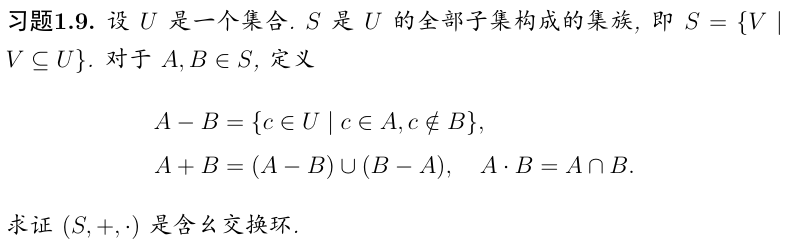
\includegraphics[width=\textwidth]{hw7-2025042722.png}
% \caption{}
\label{}
\end{figure}
$S$ is a ring and $A^2=A\cdot A=A\cap A=A$ thus $S$ is bool.
\end{proof}

\begin{exercise}
\begin{figure}[H]
\centering

\includegraphics[width=\textwidth]{2-hw7-2025042721.png}
% \caption{}
\label{}
\end{figure}
\end{exercise}
\begin{proof}
An integral domain is a commutative ring with no zero-divisor. To verify that any nontrivial finite integral domain is field, it suffices to find the inverse for every $a\in R$. Consider the ring homomorphism of additive groups
\[
\phi_{a}:(R,+)\to(R,+)\qquad x\mapsto ax
\]
The kernel $\ker \phi_{a}=\{ x\in R:ax=0 \}=\{ 0 \}$, due to the property of integral domain. Thus $\phi_{a}$ is injective, and hence is isomorphism by counting the number of elements. In particular, $a^{-1}\coloneqq \phi ^{-1}_{a}(1)$ is a multiplicative inverse of $a$. Then we are done.
\end{proof}

\begin{exercise}
\begin{figure}[H]
\centering
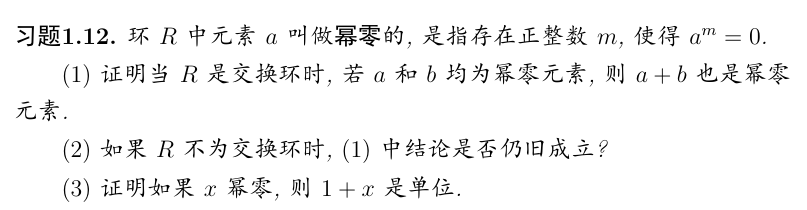
\includegraphics[width=\textwidth]{3-hw7-2025042721.png}
% \caption{}
\label{}
\end{figure}
\end{exercise}
\begin{proof}
(1) Since $a, b$ are nilpotent, there exists $m, n\in \mathbb{N}$, s.t.
\[
a^{m}=b^{n}=0
\]
Then
\[
(a+b)^{m+n}=\sum_{k=0}^{n}{\binom{m+n}{k} }a^{k}b^{m+n-k}
\]
Either $k\geq m$ or $m+n-k\geq n$ happens. Then $a^{k}b^{m+n-k}=0,\forall m, n\in \mathbb{N}$. Hence $a+b$ is also nilpotent.

(2) The conclusion in (1) may fail when $R$ is not commutative. Consider the nilpotent elements in the ring $\mathrm{Mat}_{2}(\mathbb{Z})$,
\[
a=\begin{pmatrix}
0 & 1 \\
0 & 0 
\end{pmatrix},\qquad b=\begin{pmatrix}
0 & 0  \\
1 & 0
\end{pmatrix}
\]
But
\[
a+b=\begin{pmatrix}
0 & 1 \\
1 & 0
\end{pmatrix}
\]
is invertible, not nilpotent.
\end{proof}

\begin{exercise}
\begin{figure}[H]
\centering

\includegraphics[width=\textwidth]{4-hw7-2025042721.png}
% \caption{}
\label{}
\end{figure}
\end{exercise}
A subset $I\subseteq\mathbb{Z}[\sqrt{ d }]$ is called an ideal provided that

\begin{enumerate}
	\item $\forall x, y\in I$, we have $x-y\in I$.
	\item $\forall a\in I, x\in \mathbb{Z}[\sqrt{ d }]$, we have $xa\in I$.
\end{enumerate}

\begin{proof}
Assume not, i.e. there exists an ideal $I\subseteq \mathbb{Z}\sqrt{ d }\coloneqq \{ n\sqrt{ d }:n\in \mathbb{Z} \}$. For $a=n\sqrt{ d }\in \mathbb{Z}\sqrt{ d }$, pick $x=\sqrt{ d }\in \mathbb{Z}[\sqrt{ d }]$, then $xa=nd\not\in \mathbb{Z}[\sqrt{ d }]\supset I$, which is a contradiction.
\end{proof}

\begin{exercise}
\begin{figure}[H]
\centering

\includegraphics[width=\textwidth]{5-hw7-2025042721.png}
% \caption{}
\label{}
\end{figure}
\end{exercise}
\begin{proof}
If $\phi\in \mathrm{Aut}(\mathbb{Q}[\sqrt{ d }])$ is a ring automorphism, we have
\[
\phi(1)\cdot \phi(1)=\phi(1)
\]
The equation $x^2=x$ has solution $1,0$ in $\mathbb{R}\supset \mathbb{Q}[\sqrt{ d }]$. If $\phi(1)=0$, then for any $x\in \mathbb{Q}[\sqrt{ d }]$, $\phi(x)=\phi(1\cdot x)=\phi(1)\cdot \phi(x)=0$, which means $\phi$ is not automorphism. Thus $\phi(1)=1$.

Then consider $\phi(\sqrt{ d })\eqqcolon a$, we have
\[
d=d\phi(1)=\phi(d)=\phi(\sqrt{ d })\cdot \phi(\sqrt{ d })=a^2
\]
Then $a=\pm \sqrt{ d }$.

For any $\phi\in \mathrm{Aut}(\mathbb{Q}[\sqrt{ d }])$, $\phi$ is determined by $\phi(1)$ and $\phi(\sqrt{ d })$, since for any $x+y\sqrt{ d }\in \mathbb{Q}[\sqrt{ d }]$,
\[
\phi(x+y\sqrt{ d })=x\phi(1)+y\phi(\sqrt{ d })
\]
Then
\[
\mathrm{Aut}(\mathbb{Q}[\sqrt{ d }])\cong  \{ \mathrm{id}, \alpha \}\cong \mathbb{Z}_{2}
\]
where $\alpha:a+b \sqrt{ 2 }\longmapsto a-b \sqrt{ 2 }$.

(2) For $\phi\in\mathrm{Aut}(\mathbb{Z}/m\mathbb{Z})$, it is determined by $\phi(1)$, since for any $n\in \mathbb{Z}/m\mathbb{Z}$,
\[
\phi (n)=n\phi(1)
\]
Since $\phi$ is automorphism, we have $\phi (1)\in \mathbb{Z}^{\times}_{m}$. Otherwise, $\phi(1)$ is not unit, then is zero-divisor, i.e. $\phi(n)=n\phi(1)=0$ for some $1\leq n\leq m-1$, which means $\overline{n}=0\neq \overline{n}$.

We construct an isomorphism between $\mathrm{Aut}(\mathbb{Z}_m)$ and $\mathbb{Z}_m^{\times}$,
\[
\Phi:\mathrm{Aut}(\mathbb{Z}_m)\to \mathbb{Z}_m^{\times}\qquad \phi\mapsto \phi(1)
\]
The kernel $\ker \Phi=\{ \phi:\Phi(\phi)=0 \}=\{ \phi:\phi(1)=0 \}=\{ 0 \}$ is trivial. Then $\Phi$ is injective, and hence is isomorphism by counting the number of elements. Therefore,
\[
\mathrm{Aut}(\mathbb{Z}_m)\cong  \mathbb{Z}_m^{\times}
\]
\end{proof}

\begin{exercise}
\begin{figure}[H]
\centering
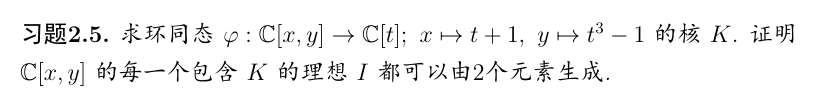
\includegraphics[width=\textwidth]{6-hw7-2025042721.png}
% \caption{}
\label{}
\end{figure}
\end{exercise}
\begin{proof}
Since
\[
y=t^{3}-1=(x-1)^{3}-1=x^3-3x^2+3x-2
\]
we have
\[
\begin{aligned}
\varphi(y-x^3+3x^2-3x+2) & =\varphi(y)-\varphi(x^3-3x^2+3x-2) \\
 & =t^3-1-[(t-1)^3-3(t-1)^2+3(t-1)-2] \\
 & =0
\end{aligned}
\]
Therefore,
\[
\left< y-x^3+3x^2-3x+2 \right>\coloneqq \{ c(y-x^3+3x^2-3x+2):c\in \mathbb{C} \}\subset \ker \varphi
\]
Since $\varphi(1)=1$ and $\varphi(x-1)=\varphi(x)-\varphi(1)=t+1-1=t$, the homomorphism $\varphi$ is surjective. Then
\[
\ker \varphi \cong \mathbb{C}[x,y]/\mathrm{Im}\varphi \cong \mathbb{C}[x,y]/\mathbb{C}[t]
\]
Consider the dimension $\dim \ker \varphi=\dim(\mathbb{C}[x,y]/\mathbb{C}[t])=1$. And
\[
\dim (\left< y-x^3+3x^2-3x+2 \right> )=1
\]
Hence,
\[
\ker \varphi=\left< y-x^3+3x^2-3x+2 \right> 
\]
Any proper ideal of $\mathbb{C}[x,y]$ containing $K$ is generated by 2 elements, otherwise it's trivial.
\end{proof}

\begin{exercise}
\begin{figure}[H]
\centering
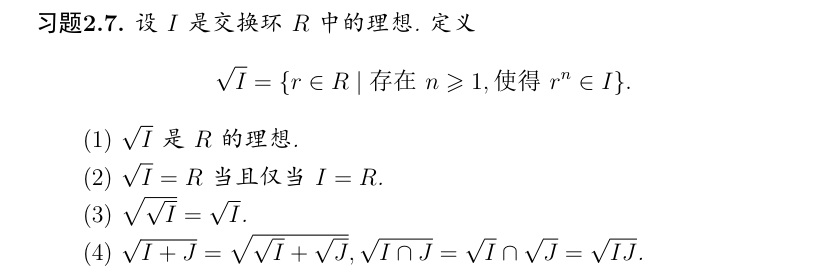
\includegraphics[width=\textwidth]{7-hw7-2025042721.png}
% \caption{}
\label{}
\end{figure}
\end{exercise}
\begin{proof}
(1)
For any $x, y\in \sqrt{ I }$, we have $x^{m}, y^{n}\in I$ for some $m,n$. Since $R$ is commutative, $I$ is a two-side ideal. Then
\[
\begin{aligned}
(x-y)^{m+n} & =\sum_{k=0}^{m+n} \binom{m+n}{k}x^{k}y^{m+n-k} \\
 & =\sum_{k=0}^{m} \binom{m+n}{k}x^{k}y^{m-k}\cdot\underbrace{  y^{n} }_{ \in I }+\sum_{k=m+1}^{m+n} \binom{m+n}{k}\underbrace{ x^{m} }_{ \in I }\cdot x^{k-m}y^{m+n-k}  \\
 & =\sum_{k=0}^{m} \underbrace{\binom{m+n}{k}x^{k}y^{m-k}\cdot  y^{n} }_{ \in I }+\sum_{k=m+1}^{m+n} \underbrace{\binom{m+n}{k} x^{m} \cdot x^{k-m}y^{m+n-k}}_{ \in I } \\
  & \in I
\end{aligned}
\]
Therefore, $x-y\in \sqrt{ I }$.

For any $x\in \sqrt{ I }, a\in R$, we have $x^{m}\in I$ for some $m$. Then
\[
(ax)^{m}=a^{m}\underbrace{ x^{m} }_{ \in I }\in I
\]
Hence $\sqrt{ I }$ is an ideal.

(2)
If $I=R$, then it's trivial that $\sqrt{ I }=R$. If $\sqrt{ I }=R$, then $1\in R=\sqrt{ I }$ implies that $1=1^{n}\in I$ for some $n$. Thus $I=(1)=R$.

(3)
Obviously, $\sqrt{ I }\subset \sqrt{ \sqrt{ I } }$. Conversely, for any $r\in \sqrt{ \sqrt{ I } }$, $r^{n}\in \sqrt{ I }$ for some $n$. Then $r^{mn}=(r^{n})^{m}\in I$ for some $m$. Hence $r\in \sqrt{ I }$. We are done.

(4)
\[
I+J\coloneqq \{ a+b:a\in I,b\in J \}
\]
\[
\sqrt{ I }+\sqrt{ J }\coloneqq \{ a+b:a^{m}\in I,b^{n}\in J,\text{ for some }m,n\geq 1 \}
\]
For $r\in \sqrt{ I+J }$, $r^{n}\in I+J\subset \sqrt{ I }+\sqrt{ J }$ for some $n$. Thus $\sqrt{ I+J }\subset \sqrt{ \sqrt{ I }+\sqrt{ J } }$. For any $r\in \sqrt{ \sqrt{ I }+\sqrt{ J } }$, $r^{s}\in \sqrt{ I }+\sqrt{ J }$ for some $s$, i.e. $r^{s}=a+b$, where $a^{m}\in I, b^{n}\in J$ for some $m,n$. Thus
\[
\begin{aligned}
r^{s (m+n)} & =(a+b)^{m+n} \\
 & =\sum_{k=0}^{m} \binom{m+n}{k}a^{k}b^{m-k}\cdot\underbrace{  b^{n} }_{ \in J }+\sum_{k=m+1}^{m+n} \binom{m+n}{k}\underbrace{  a^{m} }_{ \in I }\cdot a^{k-m}b^{m+n-k} \\
 & =\sum_{k=0}^{m} \underbrace{ \binom{m+n}{k}a^{k}b^{m-k}\cdot b^{n} }_{ \in J }+\sum_{k=m+1}^{m+n} \underbrace{ \binom{m+n}{k} a^{m}\cdot a^{k-m}b^{m+n-k}  }_{ \in I }  \\
 & \in I+J
\end{aligned}
\]
Therefore $r\in \sqrt{ I+J }$. Hence $\sqrt{ I+J }=\sqrt{ \sqrt{ I }+\sqrt{ J } }$.
\[
IJ=\{ \text{finite sums of elements }ab\text{ for }a\in I,b\in J \}
\]
If $r\in \sqrt{ I\cap J }$ then $r^{n}\in I\cap J$ for some $n$. Then $r\in \sqrt{ I }\cap \sqrt{ J }$. If $r\in \sqrt{ I }\cap \sqrt{ J }$ then $r^{n}\in I, r^{m}\in J$ for some $m,n$. Then $r^{m+n}\in I\cap J$, thus $r\in \sqrt{ I\cap J }$. Hence
\[
\sqrt{ I\cap J }=\sqrt{ I }\cap \sqrt{ J }
\]
\end{proof}

\begin{exercise}
\begin{figure}[H]
\centering

\includegraphics[width=\textwidth]{8-hw7-2025042721.png}
% \caption{}
\label{}
\end{figure}
\end{exercise}
\begin{proof}
For any $a\in R$, consider the sequence of principle ideals
\[
\left< a \right> \supset\left< a^2 \right> \supset\left< a^3 \right> \supset\dots
\]
Since the number of ideals is finite, we must have $\left< a^{m} \right>= \left< a^{m+1} \right>$ for some $m$. Then there exists $b\in R$ s.t.
\[
a^{m}=b a^{m+1}\Rightarrow a^{m}(1-ba)=0
\]
Since $R$ is integral domain, $a^{m}$ is not zero-divisor, then $1=ba$. Since $R$ is commutative, $b$ is the inverse of $a$. Due to the arbitrarity of $a$, each nonzero element in $R$ admits an inverse. Thus $R$ is a field.
\end{proof}
